Wie im vorigen Abschnitt beschrieben wurde, fehlt der bisherigen Beschreibung von Webservices der semantische Aspekt.

Die \emph{Semantik} (griechisch, "`Bezeichnung"') beschreibt das Wesen von Dingen und ermöglicht die Interpretation und Übertragung von Konzepten auf konkrete Begebenheiten. Semantik ist die Grundlage jeglicher Kommunikation und umgibt uns überall. Die semantische Bedeutung ist dabei aber kontextabhängig, das bedeutet, dass die selbe Information je nach Umgebung unterschiedlich interpretiert werden kann. In \cite[S.381]{springerlink:10.3758/BF03213193} untersuchen Halff, Ortony und Anderson die subjektive Stärke der Farbe Rot. Dabei wurden die Teilnehmer der Studie gebeten, die Stärke der Farbe in verschiedenen Sätzen zu gewichten. Die Teilnehmer gaben an, dass das Rot im Satz "`He saw red when secretary came in an hour late."' deutlich \emph{roter} ist, als im Satz "`The U.S. flag is red, white and blue"'.

Unter \emph{semantischen Webservices} versteht man solche Webservices, deren Beschreibung neben den konkreten technischen Aspekten zur Anbindung auch Information zur abgebildeten "`Welt"' enthalten. Wie schon in der Einleitung auf Seite \pageref{l:intro-loosecoupling} beschrieben, ist die semantische Beschreibung von Webservices Voraussetzung für eine Service-Infrastruktur mit loser Kopplung, denn erst so kann die Bedeutung der Aufgabe, die mit dem Webservice abgebildet wird automatisch ermittelt werden kann.

Die \ac{WSDL} ist der Standard zur Beschreibung von Webservices. Allerdings legt man damit lediglich Syntax für die vom Webservice verarbeiteten Anfragen fest. Die Bedeutung der Funktionalität und der übertragenen Daten erschließt sich daraus nicht. Sie entsteht lediglich in der Interpretation der Benutzer des Dienstes. Der \ac{WSDL} fehlt also eine Komponente, die dem reinen Akt der Datenübertragung eine inhaltliche Beschreibung hinzufügt und das zudem noch in maschinenlesbarer Form. In der Informatik sind das \emph{Ontologien}. Ontologien sind die \emph{Spezifikation eines Konzepts}. \emph{Spezifikation} bedeutet dabei eine formale und deklarative Repräsentation, die damit automatisch maschinenlesbar ist und Missverständnisse ausschließt. Ein \emph{Konzept} ist die abstrakte und vereinfachte Sicht der für das Konzept relevanten Umgebung. Ontologien beschreiben aus der Sicht des Dienstanbieters die Zusammenhänge in der Umgebung, auf die durch den Webservice implizit zugegriffen wird. In \cite[S.31]{dcswe} liefert Devedžić zum bessern Verständnis dieses Bildnis: Möchte eine Person über Dinge aus der Domäne \emph{D} mit der Sprache \emph{L} sprechen, beschreiben Ontologien die Dinge, von denen angenommen wird, dass sie in \emph{D} als Konzepte, Beziehungen und Eigenschaften von \emph{L} existieren.

\begin{figure}[ht]
\centering
\parbox{\textwidth}{
    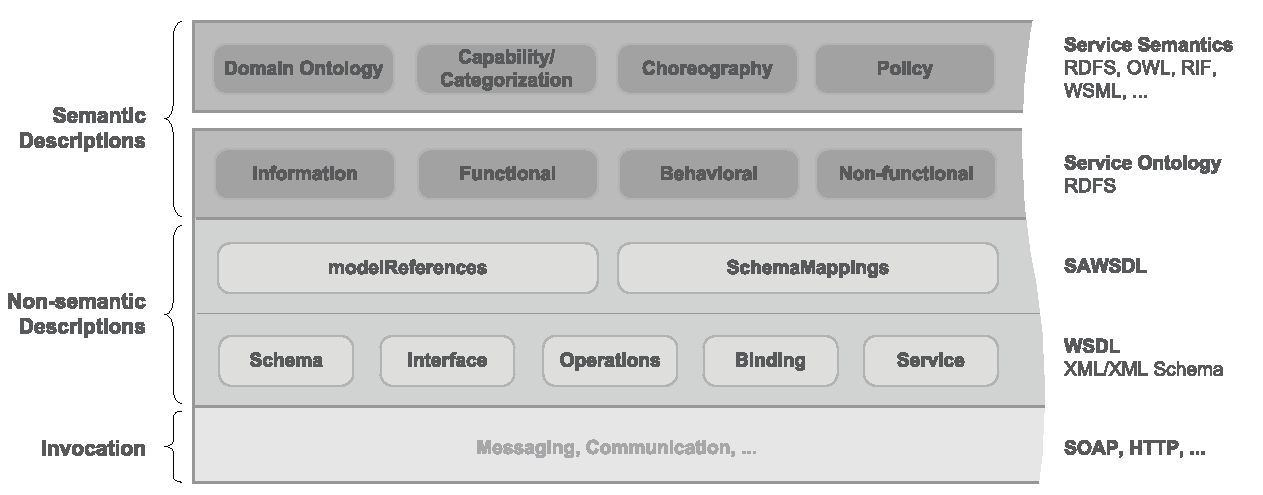
\includegraphics[width=\textwidth]{media/Extended-Web-Service-Specification-Stack.pdf}
    \caption{\emph{Extended Web service specification stack.} \cite[S.63]{ky-sawsdl}}
    \label{f:ewsss}
}
\end{figure}

\label{l:sawsdl}Mit den \ac{SAWSDL} hat das \ac{W3C} im Jahr 2007 den Entwurf eines Standard vorgelegt, der es ermöglicht Informationen zu diesen Ontologien maschinenlesbar, als Teil einer \ac{WSDL}-Datei, auszuliefern. \ac{SAWSDL} ist dabei unabhängig von einem semantischen Konzept und liefert nur den Rahmen um andere semantische Frameworks in \ac{WSDL} zu integrieren --- es wird lediglich vorausgesetzt, dass diese Konzepte anhand von URIs identifiziert werden können \cite[S.61]{ky-sawsdl}. Abbildung~\ref{f:ewsss} auf Seite~\pageref{f:ewsss} liefert einen Überblick über den Zusammenhang von \ac{SAWSDL} und den weiteren Technologien für semantische Webservices. Die Hauptbeschreibungssprache \ac{WSDL} ist dabei eng an die darunterliegenden Kommunikationsprotokolle gekoppelt. \ac{SAWSDL} verbindet als Schicht darüber \ac{WSDL} mit den übergeordneten semantischen Informationen, wobei die Service-Ontologien die allgemeinen Aspekte von Webservice beschreiben und die Service-Semantik die domainspezifischen Aspekte formuliert. Eine mögliche Technik zur semantischen Beschreibung bietet die \ac{OWL}, die auf dem \ac{RDF} basiert. In \ac{RDF} werden dabei die Entitäten (in \ac{RDF} "`Ressourcen"' genannt) mit ihren Attributen und Beziehungen untereinander syntaktisch beschrieben. In \ac{RDF} fehlt aber die Möglichkeit, die Beziehungen von Eigenschaften zu beschreiben. Zum Beispiel besitzt ein Buch das Attribut \emph{Autor} --- dass damit aber eine weitere Ressource gemeint ist (eine \emph{Person} mit der Rolle \emph{Autor}) lässt sich in einem \ac{RDF}-Dokument nicht hinterlegen. Mit der \ac{RDFS} wurde deswegen die Möglichkeit geschaffen, Gruppen zusammengehöriger Ressourcen und ihrer Beziehung untereinander zu beschreiben. Mit \ac{OWL} ist es schließlich möglich, Ontologien in Form von Klassen, Eigenschaften, Instanzen und Operationen zu beschreiben. 

\begin{figure}[ht]
\centering
\parbox{0.85\textwidth}{
    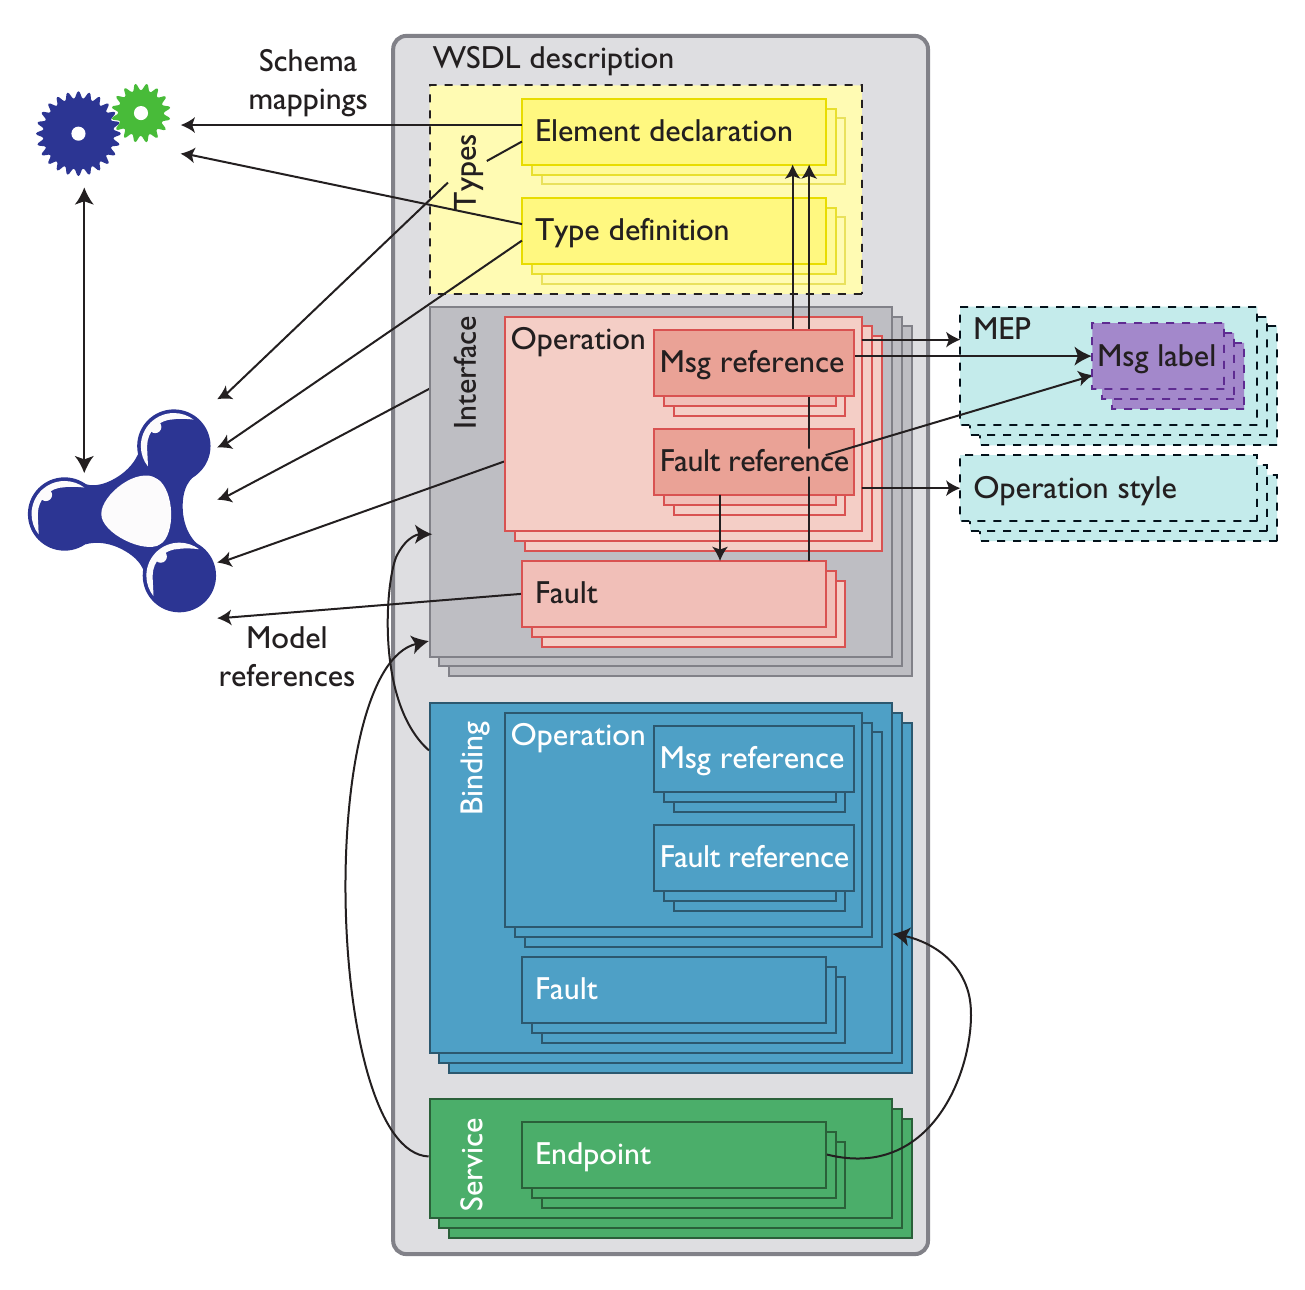
\includegraphics[width=0.85\textwidth]{media/sawsdl.png}
    \caption{\ac{WSDL} mit \ac{SAWSDL}-Erweiterungen. \cite[S.61]{ky-sawsdl}
}
    \label{f:sawsdl}
}
\end{figure}

Abbildung~\ref{f:sawsdl} auf Seite~\pageref{f:sawsdl} liefert eine Übersicht über die Integrationspunkte von \ac{SAWSDL} in \ac{WSDL}. Im Gegensatz zu semantischer Betrachtung wird \ac{WSDL} auf einer syntaktischen Ebene beschrieben. Es wird festgelegt, wie die auszutauschenden Nachrichten \emph{aussehen} und an welchen Endpunkten der \ac{API} diese zum Einsatz kommen, nicht jedoch was sie \emph{bedeuten}. Es werden die abstrakten Elemente \emph{Element Declaration}, \emph{Type Definition} und \emph{Interface} verwendet, um einen Webservice allgemein zu beschreiben. In diesen Elementen spielen die technischen Einzelheiten, wie z.B. das verwendete Protokoll, keine Rolle. Ein \emph{Type} entspricht dabei einem Objekt aus der Domäne, ein \emph{Element} beschreibt ein Attribut dieses Objekts. Ein \emph{Interface} beschreibt die Operationen und deren Parameter, die von der Schnittstelle unterstützt werden. 

\ac{SAWSDL} führt nun für diese drei Elemente zusätzlich Attribute ein, um deren semantische Bedeutung zu beschreiben \cite[S.62ff]{ky-sawsdl}. Mittels der 
\texttt{modelReference} definiert eine Beziehung zwischen einem der definierten Komponente in der \ac{WSDL} und einem Objekt im semantischen Modell. Dieses Attribut kann auf jedes \ac{WSDL}- oder \emph{XML}-Schema-Element angewendet werden. Der Wert des Attributes ist dabei eine oder mehrere URIs, die auf ein semantisches Modell verweisen. Die Attribute \texttt{liftingSchemaMapping} und \texttt{loweringSchemaMapping}, die auf Typedefinitionen definiert werden können, spezifizieren das Mapping zwischen semantischen Daten (z.B. \ac{RDF} und \emph{XML}) sowie umgekehrt. Hierbei ist es auch möglich, mehrere Mappings je Typ zu definieren, um verschiedene Repräsentationen je Kontext zu ermöglichen. Die \emph{lifting}- und \emph{lowering}-Transformationen sind nützlich, wenn von einem semantischen Client aus mit einem Webservice kommunziert wird. Für eine Anfrage werden dann die semantischen Daten in das Anfrage-Format des Clients durch \emph{lowering} transformiert, die Antwort wird dann durch \emph{lifting} wieder in ein semantisches Format konvertiert. Dieses Verfahren kommt auch bei der Verwendung einer gemeinsamen Ontologie zum Einsatz --- ein automatischer Vermittler kann dabei die Daten zwischen zwei Endpunkten mit den \emph{Lifting}-Informationen des Anfragers und den \emph{Lowering}-Informationen des Empfängers vermitteln. Sprachen für das \texttt{liftingSchemaMapping} sind z.B. \emph{XSLT} oder \emph{XQuery}, für das \texttt{loweringSchemaMapping} \emph{SPARQL} (eine Abfrage-Sprache für \ac{RDF}) gefolgt von \emph{XSLT} oder \emph{XQuery}.

\subsection*{Ausblick: RESTful Webservices}

Auch wenn dass \ac{W3C} in seinen Standards und Entwürfen keine Vorgaben zur eigentlichen Realisierung der Kommunikation mit Webservices macht, sind Standards wie \ac{WSDL} auf die Anforderungen einer \ac{SOAP}-basierten Kommunikation ausgelegt. \ac{SOAP}-basierte Webservice haben aber nur wenig mit den Strukturen des Webs gemeinsam, dort ist die vorherrschende Sprache \emph{HTTP} bei dem Ressourcen durch URIs repräsentiert werden und Aktionen durch Verben wie \texttt{GET} und \texttt{POST}. Im Gegensatz dazu versteht \ac{SOAP} einen Webservice als die \ac{API} einer Software, auf der Methode aufgerufen werden, wobei es sich zusätzlich noch um die Serialisierung und Deserialisierung der Nachrichten kümmert. Die Einfachheit eines RESTful Webservices bietet sich also gerade dann an, wenn der zugrunde liegende Dienst sowieso schon HTTP-Anfragen verarbeiten muss. \cite[S.18]{xn-sss}.

Auch die in Abschnitt~\pageref{l:einleitung} vorgestellte \ac{API} von \emph{mite} ist \emph{RESTful}. Möchte man nun aber solch eine \ac{API} semantisch beschreiben steht man vor dem Problem, dass es mit einer \ac{WSDL} nicht möglich ist eine solche Schnittstelle korrekt zu beschreiben. Dies liegt vor allem daran, dass das HTTP-Binding in \ac{WSDL} 1.1 zum einen nur \texttt{GET} und \texttt{POST} offiziell unterstützt (in \emph{REST} werden weitere HTTP-Methoden wie \texttt{PUT} und \texttt{DELETE} verwendet) und ein \emph{port type} (der Endpunkt einer API-Methode) bis zu vier verschiedene Operation pro Endpunkt definiert (Schreiben [\emph{One-way}], Schreiben \& Lesen [\emph{Request-response}], Lesen [\emph{Solicit-response}] und Benachrichtigung [\emph{Notification}]), diese aber mit der gleichen HTTP-Methode (die im \emph{binding} festgelegt wird).

\ac{WSDL} und damit auch \ac{SAWSDL} sind also ungeeignet um eine \restapi semantisch zu beschreiben, mit den Veröffentlichungen von Xuan Shi in \cite{xn-sss} und Maleshkova, Kopeck\'{y} und Pedrinaci in \cite{ma-sawslrest} stehen aber zwei Entwürfe zur Verfügung, die eine Lösung für dieses Problem bieten, deren Vorstellung aber in dieser Seminararbeit nicht behandelt wird.

\subsection{\acs{SAWSDL} verwenden}

Im vorigen Abschnitt wurde gezeigt, wie man mit Hilfe von \ac{SAWSDL} Webservices semantisch beschreiben kann. In diesem Abschnitt wird gezeigt, wie man diese Beschreibungen praktisch verwenden kann.

Der Standardisierungsprozess des \ac{W3C} fordert von allen Entwürfen für neue Standards, dass diese auf ihrer vollständige Implementierbarkeit überprüft werden müssen, bevor sie letztendlich zur Empfehlung erhoben werden dürfen. Jedes Feature der Spezifikation muss funktional in mindestens einer Implementierung vorliegen und idealerweise zwischen zwei Implementierungen interoperabel sein. Damit eine Arbeitsgruppe, also diejenigen die neue Standards entwickeln, zu einer Empfehlung kommen kann, muss diese Gruppe einen Implementierungsreport vorlegen. Im Bericht der \ac{SAWSDL}-Arbeitsgruppe\footnote{\url{http://www.w3.org/2002/ws/sawsdl/CR/}} finden sich Implementierungen in mehreren Bereichen des Standards.

Direkte Implementierungen von \ac{SAWSDL} sind Parser-\ac{API}s, die die Erweiterungen anderen Anwendungen und Werkzeugen zur Verfügung stellen, mit denen \ac{WSDL}-Dokumente semantisch beschrieben werden können. So wurde die \emph{Woden API für WSDL 2.0}\footnote{\url{http://ws.apache.org/woden/}} und die \emph{WSDL4J API für WSDL
1.1}\footnote{\url{http://sourceforge.net/projects/wsdl4j/}} so erweiterte, dass diese \ac{SAWSDL}-Informationen auslesen können. Auf diesen Bibliotheken bauen viele Jaba-basierte Werkzeuge auf, wie z.B. der Apache Webservice Stack \emph{Axis 2}\footnote{\url{http://axis.apache.org/axis2/java/core/}}. Auch zwei GUI-Werkzeuge, mit denen \ac{WSDL}-Dokumente semantisch beschrieben werden können, unterstützen den Standard: \emph{Radiant}\footnote{\url{http://lsdis.cs.uga.edu/projects/meteor-s/downloads/index.php?page=1}} von der \emph{University of Georgia} und das \acl{WSMO} \emph{Studio}\footnote{\url{http://www.wsmostudio.org/}} von \emph{Ontotext}. Da \ac{SAWSDL} wie beschrieben eine Spezifikation zum Hinzufügen von Semantiken ist, liegt sein Wert vor allem in den Anwendungen, die von diesen Semantiken gebrauch machen. Im Implementierungsreport werden mehrere solche Anwendungen erwähnt.
Insbesonderes kann man \ac{OWL-S} und \ac{WSMO}, die zu den gängigsten Frameworks für semantische Webservices zählen,  mit \ac{SAWSDL} in \ac{WSDL}-Dokumente integrieren. Mit \emph{Lumina}\footnote{\url{http://lsdis.cs.uga.edu/projects/meteor-s/downloads/Lumina/}} von der \emph{University of Georgia} können mit \ac{SAWSDL} beschriebene Webservice "`entdeckt"' werden und die \emph{Semantic Tools for Web Services}\footnote{\url{http://lists.w3.org/Archives/Public/public-ws-semann/2006Oct/0030.html}} von IBM sind in der Lage, semantische Daten zu verknüpfen und zu vermitteln.
In \ac{SAWSDL} ist es sogar möglich, semantische Beschreibungen für die \emph{Business Process Execution Language for Web Services}\footnote{\url{http://www.ibm.com/developerworks/library/specification/ws-bpel/}} (BPEL4WS) zu hinterlegen, ein Anwendungsfall der ursprünglich nicht von der Arbeitsgruppe berücksichtigt wurde. \cite[S.63]{ky-sawsdl}

Auch für die \emph{Eclipse IDE} gibt es mit \emph{Jena}\footnote{\url{http://jena.sourceforge.net/}} ein Plug-In das die Entwicklung von semantischen Webservices in Java unterstützt.

\bigskip

Wie in diesem Abschnitt gezeigt wurde, sind also die theoretischen Grundlagen und praktischen Hilfsmittel zur semantischen Beschreibung von Webservice vorhanden.
